\documentclass{report}

\usepackage{graphicx}
\usepackage{placeins}
\usepackage[obeyspaces]{url}

\begin{document}
	\begin{titlepage}
\newcommand{\HRule}{\rule{\linewidth}{0.5mm}} % Defines a new command for the horizontal lines, change thickness here

\center % Center everything on the page
 
%----------------------------------------------------------------------------------------
%	HEADING SECTIONS
%----------------------------------------------------------------------------------------

%	LOGO SECTION
%----------------------------------------------------------------------------------------
\includegraphics[width=0.5\textwidth]{logo.jpg}\\[1cm] % Include a department/university logo - this will require the graphicx package
%----------------------------------------------------------------------------------------

\vspace{2 cm}
\textsc{\large Intelligent systems programming} \\[0.4cm] % Minor heading such as course title
%----------------------------------------------------------------------------------------
%	TITLE SECTION
%----------------------------------------------------------------------------------------
\vspace{1 cm}
\HRule \\[1.0cm]
{ \LARGE \textbf{Configuration project} \small \vspace{0.4cm}}\\ % Title of your document
\HRule \\[1.0cm]
 
\center
 
\vspace{1.0 cm}

\begin{minipage}{0.4\textwidth}
\begin{centering} 
Mikkel Gaub(mikg)\\
Malthe Ettrup Kirkbro(maek)\\
Mads Frederik Madsen(mfrm)\\
\end{centering}
\end{minipage}
~
\end{titlepage}



	\section*{Overview} 
	\label{sub:overview}
	The objective of this program is to determine if a given queen placement allows for $n$ queens to be placed on a board of size $n \times n$ board without being able to attack each other.
	This is accomplished by maintaining $n^2$ variables in a BDD, each representing whether or not a queen has been placed at the corresponding board location.
	A rule for each board location is then applied, enforcing that no queen can be placed in a position vulnerable to attack from any other queen -- the \emph{board rule}.
	Another rule of the board ensures that a single queen is placed in each row -- the \emph{queens rule}.

	\section*{Board rule} 
	\label{sub:boardrule}
	The board rule is constructed by conjoining the \path{NAND}-operator between each variable and any other variable in its attack path.
	As shown in figure \ref{fig1}, this produces a BDD for each board position, preventing a queen from being in a position allowing it to attack another queen.
	
	\vspace{\fill}
	\begin{figure}[h]
		\begin{centering}
			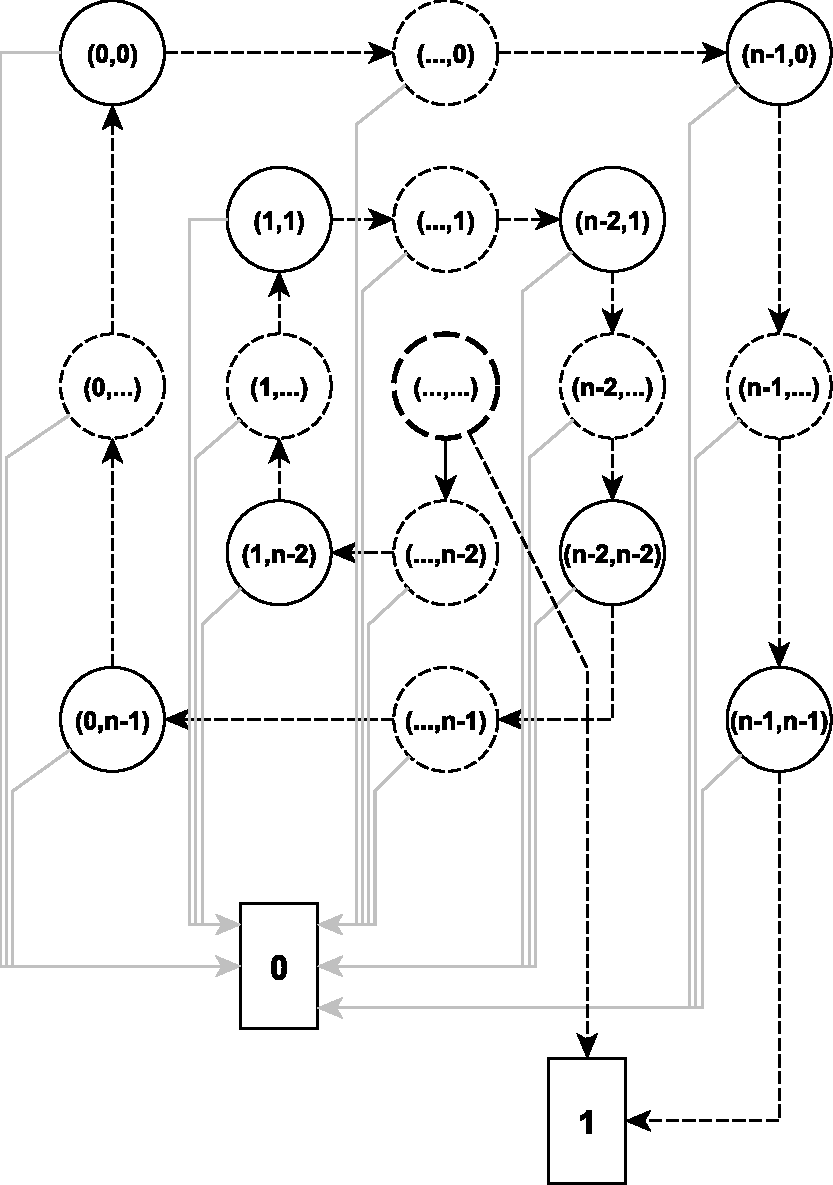
\includegraphics[width=0.5\textwidth]{figures/board-rule.pdf}
			\caption{ROBDD of the \emph{board rule} of a single queen placement in the center of a $n \times n$ chessboard. The variable ordering has been altered to give the simplest representation. The included variables are the places on the board, which are reachable from the queen's placement.}
		\end{centering}
		\label{fig1}
	\end{figure}
	\FloatBarrier

	\section*{Queens rule} 
	\label{sub:queens_rule}
	The queens rule ensures that $n$ queens are placed on the board, as each of the $n$ rows of the board must contain a queen.
	This rule is constructed by conjoining the disjunction of each position in the row for each row.
	As seen in figure \ref{fig2} this essentially guarantees that at least $n$ queens are placed on the board.
	When this rule is applied on variables already constrained by the board rule, the objective is solved.
	We can then count the number of paths through the BDD and thus determine if only one solution is possible, at which point the program automatically places the remaining queens.

	\vspace{\fill}
	\begin{figure}[h]
		\begin{centering}
			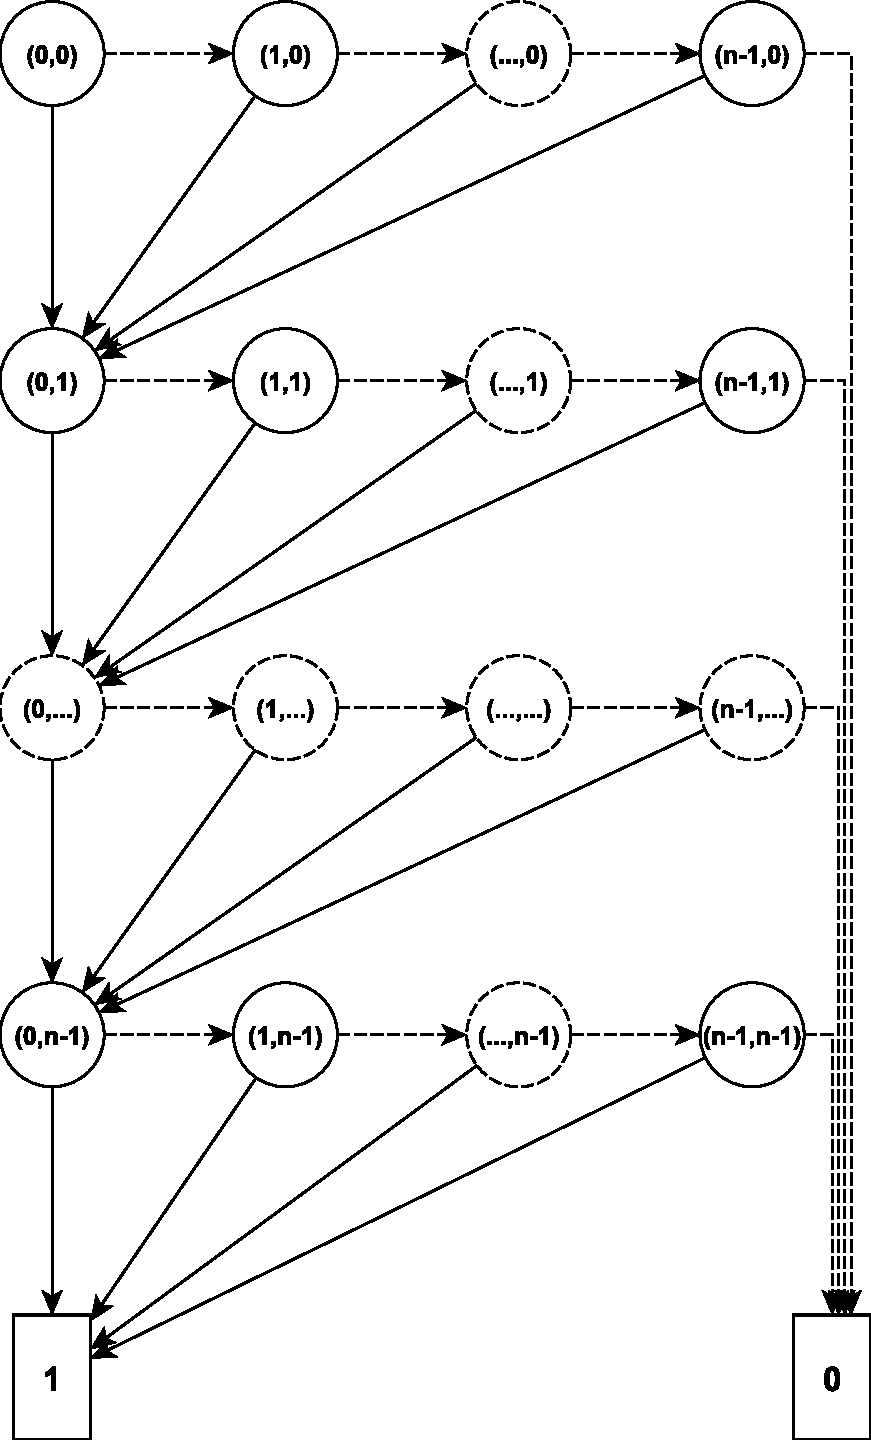
\includegraphics[width=0.5\textwidth]{figures/queen-rule.pdf}
			\caption{ROBDD of the \emph{queens rule} of a $n \times n$ chessboard. }
		\end{centering}
		\label{fig2}
	\end{figure}
	\FloatBarrier
\end{document}